% =======================================================================================
\section{Priors and the Training Distribution}
\label{app:priors}
% =======================================================================================

The flow learns $p(X\mid y, \fw)$ for the $S=\PriorsSources{}$ sources of one frequency window,
so its prior is a prior over windows: where the window sits, and what its sources are given the
window. This appendix states both, the exact symmetries of the likelihood they leave, and the
stream of simulated windows the network trains on. \Cref{fig:priors} shows the prior;
\cref{tab:priors-bands} collects what differs between the two bands.

\subsection{The Window}
\label{app:priors-window}

A window is $4R$ consecutive frequency bins of width $1/\Tobs$, with $\Tobs = \qty{\PriorsTobsYears}{\year}$, starting at an even bin $k_0 = \PriorsStride{}j$; its centre is $\fw = (k_0 +
2R)/\Tobs$. A source belongs to the window when its whole $R$-bin response fits inside it
(\cref{app:forward-model}), which confines $f_0$ to the $\PriorsInteriorResponses{}R$-bin interior, cut to
the band $[f_{\min}, f_{\max}]$:
\begin{equation}
  f_0\Tobs \in \bigl[\max(k_0 + R/2,\ f_{\min}\Tobs),\ \min(k_0 + 4R - R/2,\ f_{\max}\Tobs)\bigr].
  \label{eq:priors-interior}
\end{equation}
Training centres the window where its sources can be seen, about where the catalogue puts its
sources weighted by their chance to reach $\snr\ge k$, with $k=\PriorsVisibleSnr$:
$q(f_c)\propto p(f_c)\,P(\snr\ge k\mid f_c)$ in effect. \PriorsCandidates{} candidates
$\log_{10}f_c^{(m)}$ are drawn uniform over the band, each with one prior sky and orientation,
alone in the window centred on it at the conditional mean $\fdot$, and one is picked with weight
\begin{equation}
  w_m \propto \Normal\bigl(\log_{10}f_c^{(m)};\, \PriorsMeanF, \PriorsStdF^2\bigr)\,
  \Phi\!\Bigl(\frac{\PriorsInterceptAmp + \PriorsSlopeAmp\log_{10}f_c^{(m)} - \log_{10}\Amp_k^{(m)}}{\PriorsResidualAmp}\Bigr),\qquad
  j = \operatorname{clip}\!\Bigl(\operatorname{round}\frac{f_c\Tobs - 2R}{\PriorsStride{}},\ j_{\rm lo},\ j_{\rm hi}\Bigr),
  \label{eq:priors-window}
\end{equation}
the product of the catalogue's $f_0$ marginal (\cref{eq:priors-source}) and the chance that $\log_{10}\Amp$,
given $f_0$ (\cref{eq:priors-conditional}), exceeds $\log_{10}\Amp_k^{(m)}$, the amplitude at which that
candidate reaches $\snr=k$. The window is the one on the even grid nearest the pick, where $j_{\rm lo}$ and $j_{\rm hi}$ are the first and last windows
whose interior reaches the band. Within the window each $f_0$ follows the catalogue marginal
truncated to \cref{eq:priors-interior}, and the other parameters their catalogue priors
(\cref{app:priors-sources}). The prior given the window is therefore the catalogue's; the
weights only choose which windows training sees, so the posterior the flow learns for a window
does not depend on them.

The two bands share every prior except the band itself, and the response length $R$ that goes
with it (\cref{app:forward-model}). Windows centred on the catalogue's own $f_0$ marginal would
sit low in the band, where the sources are faint: the upper half of the full band in $\log f_0$,
which holds most of the visible sources, would get \qty{\PriorsFullTopShare}{\percent} of them, and
\qty{\PriorsFullWithVisible}{\percent} would hold a visible source. Centred by
\cref{eq:priors-window}, \qty{\PriorsFullTrainingTopShare}{\percent} of the full band's windows sit in
its upper half and \qty{\PriorsFullTrainingWithVisible}{\percent} hold a visible source
(\cref{fig:priors}d). The narrow band, below \qty{\PriorsNarrowHighMhz}{\milli\hertz}, has few
sources that can reach $k$: there the share rises only from \qty{\PriorsNarrowWithVisible}{\percent} to
\qty{\PriorsNarrowTrainingWithVisible}{\percent}. The weights are approximate, since each candidate
scores one sky and orientation alone in its window; they move the windows, not the target.

\begin{table}[t]
\caption{The two bands. Every other prior is shared. Source and window shares are over
\num{\PriorsPriorWindows} windows per band centred on the catalogue's $f_0$ marginal, and
\num{\PriorsCutWindows} centred by \cref{eq:priors-window} (training); a source is visible at
$\snr\ge\PriorsVisibleSnr$ alone in its window. Training figures are for one run of the B network
at the batch of \cref{app:priors-training}; the simulation share is the time spent drawing a batch
inside one training step on an \PriorsStepChip{}. \textcolor{red}{TODO(new bench): the full-band
step and draw times were measured at $R=1024$ and the previous prior; rerun
reports/benchmarks/step-time-memory at $R=\PriorsFullR$.}}
\label{tab:priors-bands}
\centering
\small
\begin{tabular}{lrr}
\toprule
 & narrow & full \\
\midrule
band & \qtyrange{\PriorsBandLowMhz}{\PriorsNarrowHighMhz}{\milli\hertz} & \qtyrange{\PriorsBandLowMhz}{\PriorsFullHighMhz}{\milli\hertz} \\
response $R$ / window $4R$ [bins] & \num{\PriorsNarrowR} / \num{\PriorsNarrowW} & \num{\PriorsFullR} / \num{\PriorsFullW} \\
distinct windows & \num{\PriorsNarrowWindows} & \num{\PriorsFullWindows} \\
catalogue above \qty{\PriorsCatalogueCutMhz}{\milli\hertz} in the band & \qty{\PriorsNarrowCatalogueShare}{\percent} & \qty{\PriorsFullCatalogueShare}{\percent} \\
visible sources & \qty{\PriorsNarrowVisible}{\percent} & \qty{\PriorsFullVisible}{\percent} \\
windows with a visible source, catalogue / training & \qty{\PriorsNarrowWithVisible}{\percent} / \qty{\PriorsNarrowTrainingWithVisible}{\percent} & \qty{\PriorsFullWithVisible}{\percent} / \qty{\PriorsFullTrainingWithVisible}{\percent} \\
chirp drift above one bin & \qty{\PriorsNarrowDriftOver}{\percent} of sources & \qty{\PriorsFullDriftOver}{\percent} of sources \\
\midrule
training steps & \num{\PriorsNarrowSteps} & \num{\PriorsFullSteps} \\
windows / sources seen & $\num{\PriorsNarrowObservations}$ / $\num{\PriorsNarrowSourcesSeen}$ & $\num{\PriorsFullObservations}$ / $\num{\PriorsFullSourcesSeen}$ \\
simulation share of a step & \qty{\PriorsNarrowDrawShare}{\percent} (\qty{\PriorsNarrowDrawMs}{\milli\second} of \qty{\PriorsNarrowStepMs}{\milli\second}) & \qty{\PriorsFullDrawShare}{\percent} (\qty{\PriorsFullDrawMs}{\milli\second} of \qty{\PriorsFullStepMs}{\milli\second}) \\
\bottomrule
\end{tabular}
\end{table}

\subsection{The Sources of a Window}
\label{app:priors-sources}

Given the window, the $S$ sources are drawn independently from the per-source prior of
\cref{tab:priors-source}, so they are exchangeable and the prior over a window is invariant under
their relabellings,
\begin{equation}
  \pi_w(\theta_{1:S}) = \prod_{s=1}^{S}\pi_w(\theta_s).
  \label{eq:priors-window-prior}
\end{equation}
Only $f_0$ depends on the window directly; $\fdot$ and $\Amp$ depend on it through $f_0$.

\begin{table}[t]
\caption{Prior of one source $\theta = (f_0, \fdot, \Amp, \alpha, \delta, \psi, \iota, \phi_0)$ in
window $w$.}
\label{tab:priors-source}
\centering
\small
\begin{tabular}{lll}
\toprule
parameter & prior & support \\
\midrule
$(f_0, \fdot, \Amp)$ & catalogue Gaussian in their logarithms, \cref{eq:priors-source} & \\
\quad $f_0$ & its marginal, truncated to \cref{eq:priors-interior} & $\PriorsInteriorResponses{}R$ bins at most \\
\quad $(\fdot, \Amp)\mid f_0$ & its conditional, \cref{eq:priors-conditional} & $(0, \infty)^2$, uncut \\
$(\alpha, \delta)$ & bulge, two disks and a floor in galactic $(l, \sin b)$, \cref{eq:priors-sky} & sphere \\
$\psi$ & $\Unif(0, 2\pi)$ & \\
$\iota$ & $\cos\iota\sim\Unif(-1, 1)$ & $[0, \pi]$ \\
$\phi_0$ & $\Unif(0, 2\pi)$ & \\
\bottomrule
\end{tabular}
\end{table}

\begin{figure*}[t]
  \centering
  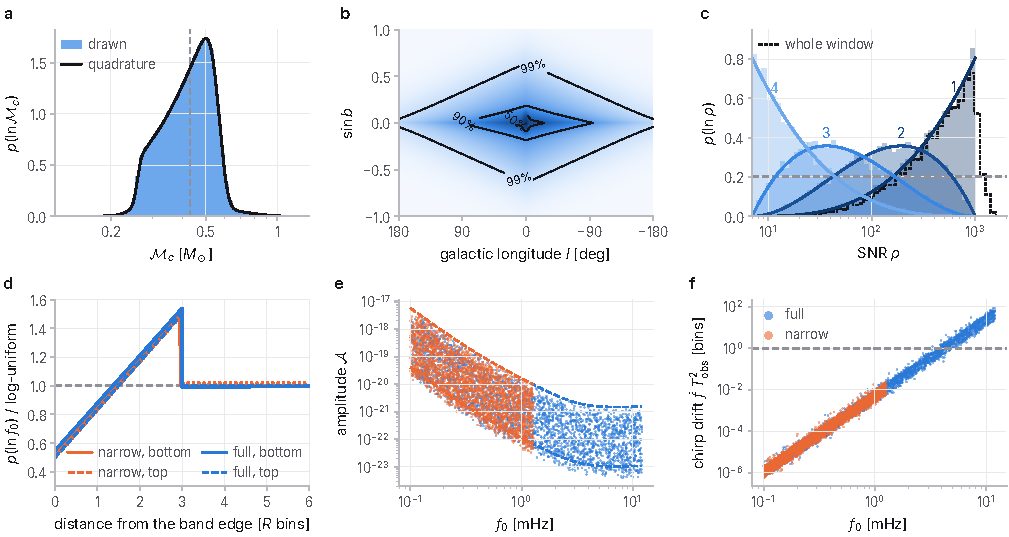
\includegraphics[width=\textwidth]{figures/priors.pdf}
  \caption{The prior over a window; lines are closed forms, filled steps and dots are
  \num{\PriorsPriorWindows} windows per band centred on the catalogue's $f_0$ marginal. (a)~$\log_{10}f_0$ of the drawn
  sources (filled) against the catalogue marginal truncated to each band (lines), and of the
  full band's visible sources, $\snr\ge\PriorsVisibleSnr$ (dashed). (b)~Sky, \cref{eq:priors-sky}, in the
  equal-area galactic $(l, \sin b)$: shading is the log density per steradian, contours enclose
  the marked share of the sources. (c)~Chirp drift over the observation, in frequency bins, in
  the full band: a sample of the sources (light), every visible one (dark), and the conditional
  mean of \cref{eq:priors-conditional} with its $\pm1\sigma$ residual (grey). Dashed: the narrow
  band's top and one bin. (d)~Where the window centres fall: on the catalogue's
  $f_0$ marginal (dashed) and by \cref{eq:priors-window} as in training (solid), per band. (e)~Amplitude, as in (c); dashed is the amplitude at which a
  source of mean-square sky and orientation reaches $\snr=\PriorsVisibleSnr$. (f)~\ac{snr} of each
  source alone in its window, per band; dashed at $\snr=\PriorsVisibleSnr$.}
  \label{fig:priors}
\end{figure*}

\paragraph{Frequency, drift and amplitude.}
$(\log_{10}f_0, \log_{10}\fdot, \log_{10}\Amp)$ is one Gaussian, fitted by maximum likelihood to
the double white dwarfs above \qty{\PriorsCatalogueCutMhz}{\milli\hertz} of a simulated Galactic
catalogue \textcolor{red}{TODO(cite): wdwd\_cat\_lam\_0p0\_alpha\_1p0\_zerotides\_MultiCGalaxy},
truncated at that cut:
\begin{equation}
  \begin{pmatrix}\log_{10}f_0\\ \log_{10}\fdot\\ \log_{10}\Amp\end{pmatrix}
  \sim \Normal(\mu, \Sigma),\qquad
  \mu = \begin{pmatrix}\PriorsMeanF\\ \PriorsMeanFdot\\ \PriorsMeanAmp\end{pmatrix},
  \label{eq:priors-source}
\end{equation}
with $f_0$ in \unit{\hertz} and $\fdot$ in \unit{\hertz\per\second}, standard deviations
$(\PriorsStdF, \PriorsStdFdot, \PriorsStdAmp)$ and correlations $\PriorsCorrFFdot$
($f_0$, $\fdot$), $\PriorsCorrFAmp$ ($f_0$, $\Amp$) and $\PriorsCorrFdotAmp$ ($\fdot$, $\Amp$). The
window truncates $f_0$ (\cref{eq:priors-interior}); the full band holds
\qty{\PriorsFullCatalogueShare}{\percent} of the catalogue above its cut, the narrow band
\qty{\PriorsNarrowCatalogueShare}{\percent}. Given $f_0$, the drift and amplitude are Gaussian with
means linear in $\log_{10}f_0$,
\begin{equation}
  \log_{10}\fdot \mid f_0 \sim \Normal\bigl(\PriorsInterceptFdot + \PriorsSlopeFdot\log_{10}f_0,\ \PriorsResidualFdot^2\bigr),\qquad
  \log_{10}\Amp \mid f_0 \sim \Normal\bigl(\PriorsInterceptAmp + \PriorsSlopeAmp\log_{10}f_0,\ \PriorsResidualAmp^2\bigr),
  \label{eq:priors-conditional}
\end{equation}
with residual correlation $\PriorsResidualCorr$. The drift slope is close to the $11/3$ of a chirp
driven by gravitational radiation, $\fdot\propto\Mc^{5/3}f_0^{11/3}$ (\cref{eq:forward-model-fdot}),
and the \PriorsResidualFdot~dex around it is the population's spread in chirp mass. $\fdot$ is a
free parameter of the source, not derived from a chirp mass, and the sampler does not cut it. Most
sources barely drift: the full band's median drift over the observation is
\PriorsFullDriftMedian{} of a bin, and \qty{\PriorsFullDriftOver}{\percent} of its sources drift
by more than one (\cref{fig:priors}c).

\paragraph{Sky.}
The sky prior is a mixture in galactic longitude $l$ and $\sin b$, the coordinates in which
$\dd l\,\dd\!\sin b$ is the solid angle:
\begin{equation}
  \pi(l, \sin b) = w_{\rm b}\,\Normal(l; 0, \sigma_l^2)\,\Normal(\sin b; 0, \sigma_b^2)
  + \sum_{d\in\{\rm thick, thin\}} w_d\,\mathcal{L}_{\pi}(l; \lambda_{l,d})\,\mathcal{L}_{1}(\sin b; \lambda_{b,d})
  + \frac{w_{\rm f}}{4\pi},
  \label{eq:priors-sky}
\end{equation}
where $\mathcal{L}_{c}(x; \lambda) \propto e^{-|x|/\lambda}$ is a Laplace density truncated to
$|x|\le c$. The bulge (widths $\PriorsBulgeScales{}$) holds \qty{\PriorsBulgeWeight}{\percent} of the weight,
the thick and thin disks (scales $\PriorsThickScales{}$ and $\PriorsThinScales{}$) hold
\qty{\PriorsThickWeight}{\percent} and \qty{\PriorsThinWeight}{\percent}, and the isotropic floor the remaining
\qty{\PriorsFloorWeight}{\percent}. The mixture was fitted to the sky positions of a catalogue of
$\num{\PriorsCatalogue}$ double white dwarfs. It traces the plane rather than the centre:
\qty{\PriorsPlaneShare}{\percent} of the sources lie within \ang{\PriorsPlaneDeg} of the galactic plane
(\cref{fig:priors}b). The forward model reads equatorial $(\alpha,\delta)$, where the galactic
centre sits at (\ang{\PriorsCentreRa}, \ang{\PriorsCentreDec}).

\paragraph{Visibility.}
The amplitude follows the catalogue, not a target \ac{snr}, so most sources lie below the noise
(\cref{fig:priors}f). A source alone in its window reaches $\snr\ge\PriorsVisibleSnr$ for
\qty{\PriorsNarrowVisible}{\percent} of the narrow band's sources and
\qty{\PriorsFullVisible}{\percent} of the full band's, and \qty{\PriorsNarrowEmpty}{\percent} and
\qty{\PriorsFullEmpty}{\percent} of windows centred on the catalogue's $f_0$ hold no visible source,
hence training's window prior (\cref{eq:priors-window}). The conditional mean
amplitude reaches the $\snr=\PriorsVisibleSnr$ amplitude of a source of mean-square sky and
orientation only above \qty{\PriorsAmpCrossMhz}{\milli\hertz} (\cref{fig:priors}e): the visible
sources are the loud tail of the top of the band. Where the data say nothing, the target posterior
is the prior, which the flow must return as faithfully as a narrow posterior.

\paragraph{A fixed number of sources.}
Every window holds exactly $S$ sources of the population. A real window holds a variable number,
most of them below any detection threshold, and a global fit infers that number with a
trans-dimensional sampler \citep{littenberg2020global}. Our flow answers the narrower question
``given that the window holds $S$ sources of the population, where are they?'', and the rest of
the population is not simulated.

\subsection{Exact Symmetries}
\label{app:priors-symmetries}

The likelihood (\cref{eq:loglik}) has two groups of exact symmetries, which a posterior sampler
must either reproduce or remove.

\paragraph{Polarisation and phase.}
A quarter turn of $\psi$ flips the sign of both polarisation tensors, and a half turn of $\phi_0$
flips the sign of both polarisations (\cref{app:forward-model}). Together they leave the signal
unchanged:
\begin{equation}
  (\psi, \phi_0) \;\mapsto\; \bigl(\psi + k\tfrac{\pi}{2},\ \phi_0 + k\pi\bigr)
  \pmod{2\pi},\qquad k = 0,1,2,3,
  \label{eq:psi-phi-symmetry}
\end{equation}
so every source's posterior has four exact copies in $(\psi,\phi_0)\in[0,2\pi)^2$. The helicity
amplitudes of the flow coordinates depend on these angles only through $\phi_0\pm2\psi$
(\cref{eq:chart}), which all four copies share: the chart folds them into one point.

\paragraph{Exchangeable sources.}
The sources are i.i.d.\ and enter the likelihood through their sum, so the
likelihood is invariant under the $S! = \PriorsPermutations{}$ relabellings: the label-switching
problem of mixture models \citep{stephens2000dealing,jasra2005markov}, which \ac{mcmc} analyses of
gravitational-wave sources meet as well \citep{buscicchio2019label}. With
\cref{eq:psi-phi-symmetry}, every mode of an unordered posterior has
$\PriorsPermutations{}\times4^{\PriorsSources{}} = \num{\PriorsCopies}$ equivalent copies. The chart folds the
phase copies, and the slots in order of $f_0$ remove the permutations (\cref{app:chart-slots}). The evaluation pairs drawn and injected sources
before scoring (\cref{app:evaluation}).

\paragraph{Approximate degeneracies.}
Amplitude trades against inclination, a distant face-on source against a nearer inclined one;
for a nearly face-on source one helicity dominates and the phase of the other is barely
constrained (\cref{app:chart-helicity}). At low frequency the chirp drift $\fdot\Tobs^2$ is a
small fraction of a bin (\cref{fig:priors}c, \cref{tab:priors-bands}) and $\fdot$ stays close to
its prior. \textcolor{red}{TODO(new chains): the median Fisher precision of $\log_{10}\fdot$ over
its prior per loudness rank, narrow against full band, from the evaluation injections under this
prior.}

\subsection{The Training Distribution}
\label{app:priors-training}

There is no fixed dataset: every training example is a freshly simulated window,
\begin{enumerate}
  \item a centre $\fw$ by \cref{eq:priors-window} and sources $\theta_{1:S}\sim\pi_w$ by
  \cref{eq:priors-window-prior};
  \item noisy data in the window's $4R$ bins and its whitened conditioning input $y$
  (\cref{app:noise});
  \item the target $X_1 = \varphi(\theta_{1:S};\fw)$ in flow coordinates, $S\times\PriorsCoords{}$,
  sources in order of $f_0$ (\cref{eq:chart});
  \item \PriorsDraws{} standard normal base points $Z_0$, each with its own flow time $t$, which
  with the frame give the paths and targets of \cref{eq:loss} (\cref{app:fm}).
\end{enumerate}
The base needs no simulation, so one example costs one simulation, of its target. A batch of
\num{\PriorsBatch} $(Z_0, t)$ pairs is $\PriorsObservationsPerStep{}$ windows times \PriorsDraws{} base
points, drawn inside the compiled training step. A run therefore sees $\num{\PriorsFullObservations}$ to $\num{\PriorsNarrowObservations}$ independent
windows (\cref{tab:priors-bands}): overfitting is not a concern, and every comparison between runs
is one of optimisation, not of generalisation. The simulation is cheap next to the network,
\qty{\PriorsNarrowDrawShare}{\percent} of a step in the narrow band and \qty{\PriorsFullDrawShare}{\percent} in the full band, where each response
spans \num{\PriorsFullR} bins instead of \num{\PriorsNarrowR} (\cref{app:training}).
\textcolor{red}{TODO(new bench): full-band share at $R=\PriorsFullR$.}
